\documentclass[conference]{IEEEtran}

\IEEEoverridecommandlockouts
\newcommand{\funding}{%
  This work is partially supported by the European Union under grant nos. FP7-604102 (HBP), FP7-287701 (BrainScales-Extension), and ERC-320689 (BIMPC), and by grant EP/G015740/1 (BIMPA).
}

%% Document properties (~ is a non-breaking space)
\title{Using Factored~Weight~Matrices for an efficient SpiNNaker implementation of the Neural~Engineering~Framework}
\author{%
  \IEEEauthorblockN{Andrew~Mundy and James~Knight}
  \IEEEauthorblockA{School of Computer Science,\\
                    University of Manchester,\\
                    Oxford Road, Manchester,\\
                    M13 9PL, UK\\
                    Email: andrew.mundy@ieee.org}
  \and
  \IEEEauthorblockN{Terrence~C.~Stewart}
  \IEEEauthorblockA{Centre for Theoretical Neuroscience,\\
                    University of Waterloo,\\
                    Waterloo, ON,\\
                    Canada N2L 3G1\\
                    Email: tcstewar@uwaterloo.ca}
  \and
  \IEEEauthorblockN{Steve~B.~Furber}
  \IEEEauthorblockA{School of Computer Science,\\
                    University of Manchester,\\
                    Oxford Road, Manchester,\\
                    M13 9PL, UK\\
                    Email: steve.furber@manchester.ac.uk}
  \thanks{\funding}
}

%% Utilities
\usepackage{booktabs}  %% Pleasant tables
\usepackage[binary-units]{siunitx}
\usepackage[caption=false, font=footnotesize]{subfig}
\usepackage{graphicx}
\usepackage[mode=buildnew]{standalone}

%% Source highlighting
\usepackage{listings}
\lstset{
  language=Python,
  morekeywords={with,as},
  columns=flexible,
  gobble=2,
  basicstyle=\footnotesize,
  xleftmargin=1em,
}

%% Maths
\renewcommand{\vec}{\mathbf}  % Bold vectors

%% Bibliographies
\usepackage[backend=bibtex, style=ieee, doi=false, url=false, maxbibnames=7]{biblatex}
\bibliography{paper}
\usepackage{xcolor}

\begin{document}
  \maketitle

  \begin{abstract}

Building and simulating neural systems is a promising avenue in our search for understanding how the brain may work and for how neural and cognitive systems may be employed to tackle engineering problems. The Neural Engineering Framework (NEF) is an interesting hypothesis about how such systems may be constructed and has recently being used to build the world's first functional brain model. However, while the NEF simplifies the design of complex neural networks, simulating these using standard computer hardware is still computationally expensive -- often running far slower than biological real-time and scaling very poorly: problems the SpiNNaker neuromorphic simulator was designed to solve. In this paper we (1) argue that employing the model of computation used for simulating general purpose spiking neural networks on SpiNNaker for NEF models is sub-optimal, and (2) provide and evaluate an alternative simulation scheme which overcomes the memory and communication challenges posed by the NEF.

  \end{abstract}

  \section{Introduction}

For a given power budget, two factors limit the simulation of neural networks on any computing platform: scale and time. In principle any scale of network may be simulated but as scale increases simulation time follows.
Conversely, if the simulation time is limited (for example, if biological real-time is necessary) then only a limited scale of network may be simulated. Specialised ``neuromorphic'' hardware tries to avoid these constraints by parallelising and distributing computational effort and relying on dense interconnection of the computing elements.
The SpiNNaker platform \parencite{Furber2014} is one of a range of neuromorphic simulators (including Neurogrid \parencite{Benjamin2014}, BrainScaleS \parencite{Schemmel2010} and lately TrueNorth \parencite{Merolla2014}) which should benefit investigators of embodied cognition and researchers of large neural models alike by enabling scalable, rapid simulation of large-scale neural networks.

The Neural Engineering Framework (NEF) \parencite{Eliasmith2004} is a hypothesis about how neurons may act to encode the abstract mathematical constructs, such as scalars and vectors, that we often use in modelling the real world. Its successes so far include the Spaun model of cognition \parencite{Eliasmith2012} and applications in embedded robotics (e.g., \parencite{Stewart2015ip}). As with all neural systems, the NEF has proven costly to simulate with simulations of the Spaun model typically taking \SI{2.5}{\hour} of simulation time for \SI{1}{\second} of simulation \parencite[\S V]{Stewart2014}. Two aspects of NEF networks that make them particularily costly to simulate are the high firing rates of individual neurons (around \SIrange{200}{400}{\hertz} when saturated) and the dense synaptic matrices used to connect neuronal populations. The former presents a significant communication cost to any specialised neuromorphic hardware and the latter requires that large amounts of memory be used to represent the neural network with all the associated costs of transferring large blocks of data that implies.

  In this paper we:
  \begin{enumerate}
    \item argue that due to these properties of the NEF, the existing solutions and algorithms used to simulate neural networks on SpiNNaker will not satisfactorily scale to Spaun-like models,
    \item detail a method by which features of the NEF may be used to reduce the communication and memory costs associated with its simulation.
  \end{enumerate}

The result is a model of computation similar to the data-flow computer which we hope to use in running the full Spaun model in biological real-time.

  \section{Background}

In this section we briefly discuss the SpiNNaker platform and how neural networks are currently simulated on it before introducing the Neural Engineering Framework (NEF) and discussing how models built with it may act to stress SpiNNaker in various ways.

  \subsection{The SpiNNaker platform}

The SpiNNaker platform is a massively parallel architecture designed to simulate neural networks. A SpiNNaker machine is constructed from a number of SpiNNaker chips, each connected to their six immediate neighbours using a chip-level interconnection network with a toroidal, triangular mesh topology. Each SpiNNaker chip contains 18 ARM processing cores connected, via a network-on-chip, to each other and the external network through a multicast router. Each core has two small tightly-coupled memories: \SI{32}{\kibi\byte} for instructions~(ITCM) and \SI{64}{\kibi\byte} for data~(DTCM) and shares \SI{128}{\mebi\byte} of off-chip SDRAM with the other cores on the SpiNNaker chip.

SpiNNaker is an event-driven message-passing computing architecture. The software running on a core may transmit packets to other processing cores to indicate the occurrence of events or to share data. A packet consists of a \SI{32}{\bit} key -- which is used to direct the packet around the network -- and, optionally, a \SI{32}{\bit} data payload. When a packet reaches a router the key is inspected to determine to which (if any) of the 18 processors and six external links attached to the router it should be forwarded. On receipt of a packet a core executes a \textit{callback} function which may inspect the packet and schedule further execution as required.

  \subsection{Simulating neural nets on SpiNNaker}
  \label{sef:background/nn}

When simulating neural nets on a SpiNNaker machine, each core is responsible for simulating a number (in the order of a few hundred) of point neurons. When one of these neuron spikes, it transmits a packet whose key uniquely identifies the neuron (for this it requires no payload). This ``spike'' packet is then routed across the network fabric to the processing cores responsible for simulating each of the neurons that are synaptically connected to the firing neuron. On receipt of a ``spike'' packet, a core retrieves the row of the connectivity matrix associated with the firing neuron from SDRAM. Each of these rows describes the synaptic weights and delays associated with the connections between the firing neuron and those simulated on the core. Once a row is retrived, the weights are inserted into an input ring-buffer where they remain until the synaptic delay has elapsed and they are used to calculate the neuronal input current.

There are three primary constraints to the number of neurons that may be simulated on a single processing core:

  \begin{enumerate}
    \item The amount of memory required to store the synaptic weight matrices must fit within the space available to the core.
    \item The number of packets likely to be transmitted by the core should not lead to saturation of the interconnection network.
    \item As \textcite{Sharp2013} discuss, the majority of processing time is spent in the synaptic processing pipeline so there must be sufficient time for the core to process all incoming `spike' packets; and retrieve and process the synaptic rows during one simulation time-step.
  \end{enumerate}

These constraints may be met by either allocating fewer neurons to each processing core or by increasing the processing time used for each simulation time-step.

In practice there are limits to the number of processors and the amount of time that are available (though one aim of the SpiNNaker project is to build a machine consisting of one million cores). Hard time constraints are necessary when SpiNNaker is required to run in biological real-time, as it is in experiments with other neuromorphic hardware. Processor constraints are present for those with access to only small SpiNNaker machines. At some point it is necessary to ensure that efficient use is made of the machine with regard to both time and processor usage.

To a first approximation the first constraint is that the synaptic matrices for a core's neurons must fit within $\frac{128}{16} = \SI{8}{\mebi\byte}$. The interconnection network was designed around an expectation that each core would simulate around \num{1000} neurons firing at roughly \SI{10}{\hertz} and that consequently the second constraint is that when simulating on a millisecond time-step in biological real-time each core is expected to transmit around 10 spikes per time-step. The third constraint is given by \textcite[\S III.C]{Sharp2013} as around \num{5000} spikes per millisecond.

It should be noted that time is also a factor \textit{prior} to the start of any simulation. All data required by the SpiNNaker machine during simulation must be transmitted to it across ethernet, consequently the more data required on the machine the greater the time required to prepare it for simulation. \textcite{Sharp2013} note that this can take a significant period of time and that this is undesirable if a real-time simulator is desired.

  \subsection{The Neural Engineering Framework}
  \label{sef:background/nef}

The Neural Engineering Framework (NEF) extends the concept of ``preferred-direction vectors'' \parencite{} to all neural populations. Each population represents a vector within a particular space (typically a hypersphere) and within that population, each neurons firing rate reflects the similarity of the represented vector to its own ``encoding'' vector. Using the notation of \textcite{Stewart2014} this may be expressed as:

\begin{equation}
  \delta_{i}\left(\vec{x}\right) = G_{i}\left[ \alpha_i \vec{e}_i \cdot \vec{x} + J^{bias}_i \right]
  \label{eq:encoding}
\end{equation}

Which states that the firing response of neuron $i$, $\delta_i$, to the represented value of $\vec{x}$ is the response of the neuron model ($G_{i}$) to an input consisting of a randomly selected gain term ($\alpha_i$), the neurons encoding vector ($\vec{e}_i$) and a fixed bias current $J^{bias}_i$. The process of ``encoding'' allows us to transform a variable in vector form into the spiking response of a population of neurons. Correspondingly, ``decoding'' allows a transformation from the spiking actions of neurons into the domain of vectors. Again using the notation of \textcite{Stewart2014} we can express this decoding process as:

\begin{equation}
  \vec{\hat{x}} = \sum\limits_{i=1}^{N} a_i(\vec{x})\vec{d}_i  \label{eq:decoding}
\end{equation}

Where the estimate of the original represented value $\vec{\hat{x}}$ is the sum of the spiking activity of each neuron $a_i$ multiplied by the linear decoder for the neuron $\vec{d}_i$. The decoding vectors $\vec{d}_i$ may be selected to compute a function of the value represented by the population. \figurename \ref{fig:background/nef-1} illustrates the encoding of a two-dimensional value using four neurons -- the role of the encoding vectors can be seen in that each neuron becomes active for only a small range of the input space.

  \begin{figure}[!t]
    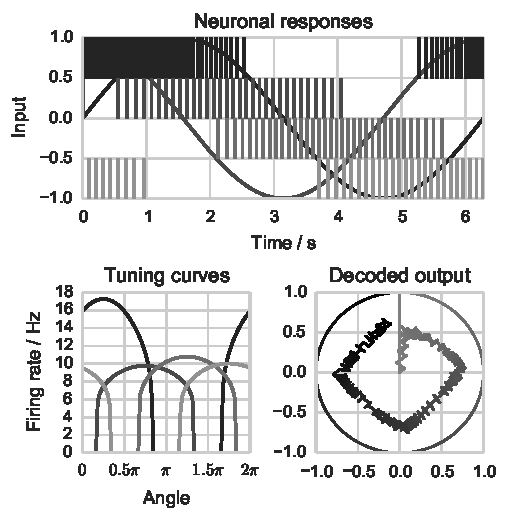
\includegraphics{figures/nef-1}
    \caption{Representing a 2-dimensional value using four neurons. The input values and spiking responses of the neurons are shown in the top plot. The bottom left-hand plot shows how the firing responses vary to the angle of the 2-D input vector (tuning curves) and the bottom right-hand plot shows a decoding of the population's representation along with the input value.}
    \label{fig:background/nef-1}
  \end{figure}

%% Synaptic filtering
For a connection between a pair of populations, a, typically dense, synaptic weight matrix can be calculated by taking the matrix product of the pre-synaptic populations decoders and the post-synaptic populations encoders \parencite{Stewart2014}:

\begin{equation}
  \omega_{ij} = \alpha_j \vec{d_i}\vec{e_j}
\end{equation}

With $i$ indexing neurons in the pre-synaptic population and $j$ those in the post-synaptic population.

  \subsection{Assessing the Neural Engineering Framework (NEF)}

As discussed in \S\ref{sef:background/nef}, it is entirely possible to translate models built using NEF principles into populations of point neurons, connected with dense synaptic weight matrices. These networks could then, in theory, be simulated using the standard SpiNNaker spiking neural network simulator described in \S\ref{sef:background/nn}. However, in this section, we show that, based on parameters used in the Spaun functional brain model, this approach would be sub-optimal when the constraints of the SpiNNaker platform outlined in \S\ref{sef:background/nn} are taken into account.

The Spaun model is built using the Semantic Pointer Architecture (SPA) \parencite{eliasmith2013build} which uses randomly chosen NEF unit vectors to represent basic concepts ($MOUSE$, $CHEESE$, $SUBJECT$, $OBJECT$, $EAT$, $VERB$). These concepts can then be combined into symbol structures using addition~($+$) and circular convolution~($\otimes$) operators, both functions being performed which are evaluated using the NEF. The circular-convolution operator is non-linear and, Eliasmith \parencite{eliasmith2013build} demonstrates, require around 70 neurons per-dimension to calculate accurately.

Using basic concepts represented as vectors and the two operators, a semantic pointer representing the sentence ``Mice eat cheese'' can be calculated as $S=MOUSE \otimes SUBJECT + EAT \otimes VERB + CHEESE \otimes OBJECT$. The subject of this sentence could then be extracted using $S \otimes SUBJECT^{-1} \approx MOUSE$. However, this later process is relatively noisy, meaning that, in order to extract the $MOUSE$ semantic pointer, the result needs to be ``cleaned up''. This process is performed using an auto-associative memory network \parencite{Stewart2011}, the properties of which dictate that in order to reliably extract a human-scale lexicon from a semantic pointer, it requires around 500 dimensions.

On the basis of these two parameters, we can determine that, functions on these vectors must be evaluated using $3.5\times10^4$ neuron populations, two of which would be connected using a dense synaptic matrix with $1.225\times10^9$ entries. Synapses on SpiNNaker are typically represented as \SI{32}{\bit} values, meaning that the synaptic matrix would be approximately \SI{4.5}{\gibi\byte}. This means that, as each core only has \SI{8}{\mebi\byte} of SDRAM, each of these populations would have to be distributed between 585 cores, reducing the number of neurons simulated per core to only 53 -- Several orders of magnitude short of SpiNNaker's architectural target of 1000 \parencite{}. 

%* Each core only left simulating 59 neurons - Design target 1000 **CITE**
%* 42373 cores to fit Spaun = 2649 chips = 56 48-node SpiNNaker boards
%
%Incoming spikes - 5000/ms
%--------------------------
%* Each of these cores would have 2*10^6 synapses
%
%Outgoing spikes - 10/ms
%------------------------

  \subsection{Constructing models with the NEF}

Neural models built using the principals of the NEF may be implemented in any programming language, however, a standard Python library for building and simulating these models has been developed. Nengo \parencite{Bekolay2014} provides several core components which may be used to specify models for simulation:

  \begin{description}[\IEEEsetlabelwidth{Connections}]
    \item[Ensembles] A population of neurons with their attendant encoders.
    \item[Nodes] General purpose non-neural components, typically used to inject values into simulations or to drive real-world actuators.
    \item[Connections] Specify how nodes and ensembles are connected.
    \item[Probes] Allow gathering of simulation data for later analysis.
  \end{description}

  An illustrative model that we will use later in this paper is the \textit{communication channel}. A communication channel consists of two ensembles connected with the synaptic weights chosen such that the second ensemble will represent the same value as the first ensemble. The concept is illustrated in \figurename~\ref{fig:background/comms-channel}. Using Nengo a communication channel may be constructed as:

  \begin{lstlisting}
  with nengo.Network('Communication Channel') as comms_channel:
      # 2 100 neuron ensembles, each of 2-dimensions
      ens_a = nengo.Ensemble(100, 2)
      ens_b = nengo.Ensemble(100, 2)

      # Connection from A to B with the identity function
      nengo.Connection(ens_a, ens_b)
  \end{lstlisting}

  \begin{figure}
    \centering
    \includestandalone{figures/comms_channel_map}
    \caption{A NEF communication channel consisting of two populations of neurons and a connection.
             The diagram indicates how the abstract communication channel might be instantiated on a simplified representation of the SpiNNaker architecture:
             Population $A$ is split between processing two cores, consequently two streams of multicast packets allow simulation of the communication channel.
    }
    \label{fig:background/comms-channel}
  \end{figure}

  \section{Exploiting features of the NEF for effective simulation on SpiNNaker}

  Previous sections have illustrated how use of the NEF can be expected to result in networks which are not amenable to efficient implementation using the standard SpiNNaker paradigm.
  In this section we review an alternative simulation scheme that will meet the constraints of the SpiNNaker hardware for a large range of networks constructed using the NEF.
  The NEF permits us two different views of the activity of a neural population: that of spikes and that of a set of time-varying vectors.
  In our simulation scheme we use the second of these to facilitate communication of neural activity between processing cores.

  We split the execution time of a processing core into three steps: \textit{input filtering}, \textit{neuron update} and \textit{output}.
  In the old simulation scheme the ``inputs'' to a processing core were in the form of ``spike'' packets which were used to drive a pipeline which retrieved synaptic weights from SDRAM; in our new scheme the inputs take the form of a set of packets whose payloads can be combined to form a vector.
  For example, the processing core simulating population $B$ from \figurename~\ref{fig:background/comms-channel} will receive two packets per time-step from each of the two cores simulating population $A$ -- combining these packets will form a 2-D vector representing the current decoding of the activity of $A$.
  At the start of each simulation step the values which were received in this manner are filtered using the appropriate synaptic filter model and then summed to form a single vector which is the current input to the population -- this forms the \textit{input filtering} step.

  During the \textit{neuron update} step the state of each neuron is updated in turn.
  First the input for the neuron is computed by calculating the dot product between the encoding vector for the neuron and the current input to the population ($\alpha_i \vec{e}_i \cdot \vec{x} + J^{bias}_i$ from (\ref{eq:encoding})).
  Then the neuron itself is simulated, for example using the Euler method to compute the next state of a LIF neuron.
  If, during this process, a neuron spikes then its decoding vector ($\vec{d}_i$) is looked up and added to a buffer containing the current decoding of the population activity (as in (\ref{eq:decoding})).
  Once all the neurons have been simulated the output buffer contains a vector which represents the weighted decoding of any spikes which occurred during the simulation step.

  During the \textit{output} stage each element of the output buffer vector is transmitted in the payload of a multicast packet with a key which uniquely identifies the population, decoding vector and element index.
  The communication fabric routes these ``value'' packets to cores which simulate connected populations of neurons.

  Some ensembles may have multiple outgoing connections with different transformations or functions, as a result there are multiple decoder matrices which need to be applied when decoding the activity of the population.
  In these cases we combine the matrices such that the decoding vector for any neuron is the concatenation of the required decoders
  (i.e., $\vec{d}_i = \left[\vec{d}_i^{f(\vec{x})},\,\vec{d}_i^{g(\vec{x})},\,\ldots \right]$).

  \section{Results}
  \label{sec:results}

  \subsection{Processor utilisation}

  \textbf{Processor utilisation for communication channel (show variation with dimensionality and neuron count) \color{red} Jamie}

  \begin{figure}[!t]
    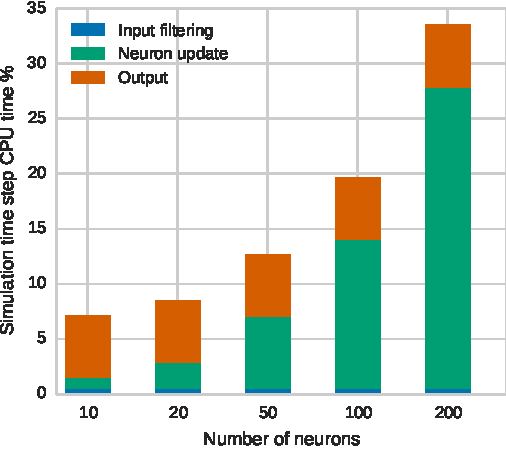
\includegraphics{figures/comm_channel_cpu_16d_bar}
    \caption{}
    \label{fig:results/comm-channel-cpu-16d}
  \end{figure}

  \begin{figure}[!t]
    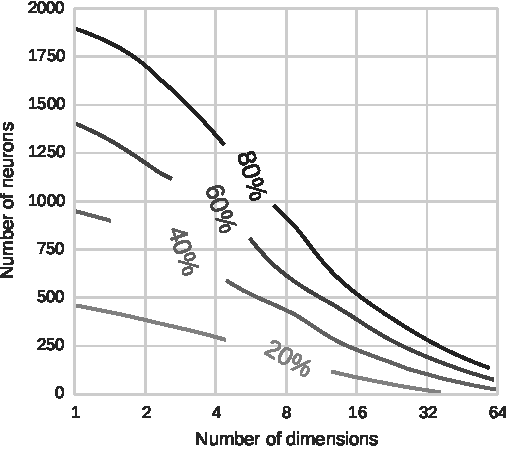
\includegraphics{figures/comm_channel_cpu_contour}
    \caption{}
    \label{fig:results/comm-channel-cpu-contour}
  \end{figure}
  
  \subsection{Network utilisation}

  \textbf{Network utilisation for communication channel, varying neuron count and dimensionality \color{red} Andrew}

  \begin{figure}[!t]
    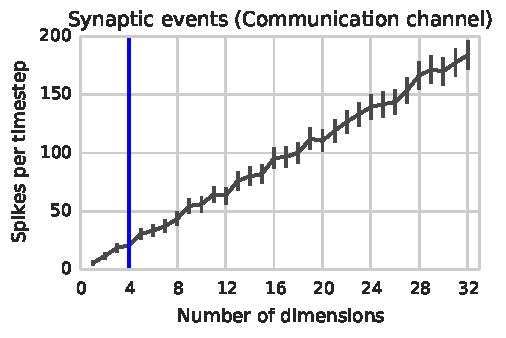
\includegraphics{figures/network-1}
    \caption{}
    \label{fig:results/network-utilisation}
  \end{figure}

  \subsection{Memory utilisation}

  \textbf{Memory utilisation for comms channel and basal ganglia model with varying scale \color{red} Andrew}

  \subsection{Simulating large-scale models}
  \label{sec:spa-sequence}

  \textbf{Simulation results from SPA sequence, indicate compute/load time \color{red} Both, discuss first.}

  \section{Discussion}

  \subsection{Comparison to prior SpiNNaker implementations}

  \textcite{Galluppi2012} demonstrated a mapping from models written in Nengo to the SpiNNaker architecture using the older simulation method described in \S\ref{sef:background/nn}.
  This implementation also used the encoding/decoding processes to reduce communication overheads between computational elements, but, unlike the method presented here, only applied it to communication between SpiNNaker and an external computer.
  Instead, use of spike-based transmission necessitated the storage of complete weight matrices and led to a significant amount of time being required to transfer simulation data to the SpiNNaker machine, \citeauthor{Galluppi2012} suggested that this may be overcome by transmitting encoders and decoders separately and performing the matrix multiplication on SpiNNaker.
  This would have reduced the load time but would not have solved the problem of the synaptic matrices filling the usable memory, nor the associated issues of spike rates and network usage.
  For the reasons advanced above we believe that this implementation of the NEF on SpiNNaker would not have satisfactorily scaled to simulate models of the scale or complexity of Spaun.

  \subsection{Comparison to other neuromorphic simulators}

  SpiNNaker is but one of a range of neuromorphic simulators, a family including both analogue (e.g., Neurogrid \parencite{Benjamin2014}, BrainScaleS \parencite{Schemmel2010}) and digital (e.g., TrueNorth \parencite{Merolla2014}) hardware, which aim to reduce the power consumption and execution time for simulating large neural models.
  Of these, the analogue simulators can be expected to require less power than SpiNNaker for a given scale of model \parencite{Stromatias2013} and to be able simulate faster than biological real-time; however, they are limited to simulating neurons and synapses of the type cast in silicon whereas SpiNNaker may be reprogrammed as required to investigate new models and learning rules.

  \subsection{Comparison to general purpose computer simulators}

  \S\ref{sec:spa-sequence} illustrated how the SpiNNaker compared to the Python implementation of Nengo when simulating models of a communication channel and a more complicated example highlighting features of the NEF and SPA.
  For some scales of models it may be expected that the overheads of specialised hardware (including SpiNNaker) are sufficiently great that simulation on standard computing hardware and GPUs can be expected to be faster.
  When this is the case, the Python implementation of Nengo of \textcite[\S6]{Bekolay2014} is shown to compare favourably with several standard neural simulators (Brian \parencite{Goodman2009}, NEURON \parencite{Hines2009} and NEST \parencite{Eppler2009}) on a range of networks, and an OpenCL implementation of Nengo is shown to perform even better but is only demonstrated on feed-forward networks.
  However, when simulating models on the scale of Spaun we expect the simulation scheme detailed in this paper to provide substantial speed improvements over standard computing hardware even when the overheads are taken into account; moreover as SpiNNaker is a real-time simulator we expect it to perform well in conjunction with neuromorphic sensors or actuators.

  \subsection{General applicability of the algorithm}

  SpiNNaker is a example of a message passing architecture -- consequently we expect that our simulation scheme, transmitting decodings of ensemble activity rather than spike activity, to be equally applicable to simulating neural nets on any message passing distributed architecture.
  Despite this the particular advantages of SpiNNaker (low-power and real-time) suggest that it is a good choice of platform on which to simulate large-scale neural models.

  \subsection{Future work}

  This work has laid the basis for simulating truly large-scale models built using the NEF in biological real-time.
  Several improvements are planned which should enable a greater number of neurons to fit on a single core and we anticipate the implementation of further neuron and synapse models.
  In particular, our current implementation only allows for one encoder per neuron and this is likely to be limiting in light of learning rules (e.g., \parencite{Voelker2014}) which act to modify weights in encoders.
  We also intend to better assess the computational cost or gain of value-based transmission on implementing learning rules and a constant traffic pattern affects the SpiNNaker network architecture.

  \section{Conclusion}

  This paper has shown how several properties of the NEF lead to inefficient use of the SpiNNaker computing architecture.
  We have described and assessed an alternative approach to simulating models built using the NEF on SpiNNaker that enable it to exceed the design target of 1000 neurons per core without exceeding the network capacity or becoming memory bound.
  Our intent is to use this new implementation of the NEF for SpiNNaker to simulate the full Spaun-model in biological real-time, and to investigate models of greater scale and complexity.

  \section*{Acknowledgements}

The authors would like to extend their thanks to the organisers of the Telluride Neuromorphic Cognition Engineering Workshop.

  \printbibliography

\end{document}
